%%%%%%%%%%%%%%%%%%%%%%%%%%%%%%%%%%%%%%%%%%%%%%%%%%%%%%%%%%%%%%%%%%%%%%%%%%%%%%

\documentclass{l3deliverable}

%%%%%%%%%%%%%%%%%%%%%%%%%%%%%%%%%%%%%%%%%%%%%%%%%%%%%%%%%%%%%%%%%%%%%%%%%%%%%%

\usepackage{graphicx}%
%


\version{1.0}


\usepackage{tabularx}%
\usepackage{url}%
\usepackage{usecasedescription}%

%%%%%%%%%%%%%%%%%%%%%%%%%%%%%%%%%%%%%%%%%%%%%%%%%%%%%%%%%%%%%%%%%%%%%%%%%%%%%%
%% Check these macro values for appropriateness for your own document.

\title{Requirements Document}

\author{Michael Kilian\\
	Dan Tomosoiu\\
	Tony Lau\\
	Peeranat Fupongsiripan\\
	Hector Grebbel
}

\date{31 October 2012}

\deliverableID{D3}
\project{PSD3 Group Exercise 1}
\team{L}

%%%%%%%%%%%%%%%%%%%%%%%%%%%%%%%%%%%%%%%%%%%%%%%%%%%%%%%%%%%%%%%%%%%%%%%%%%%%%%

\begin{document}

%%%%%%%%%%%%%%%%%%%%%%%%%%%%%%%%%%%%%%%%%%%%%%%%%%%%%%%%%%%%%%%%%%%%%%%%%%%%%%

\maketitle

\tableofcontents

\newpage

%%%%%%%%%%%%%%%%%%%%%%%%%%%%%%%%%%%%%%%%%%%%%%%%%%%%%%%%%%%%%%%%%%%%%%%%%%%%%%
%% Standard section for all documents

\section{Introduction}
Software Engineering (SE) and Electronic and Software Engineering (ESE) students in the School
of Computing Science are required to complete an internship as part of their course, in the summer
between level 3 and level 4. An internship is a short period of time that a student spends working
within in a company in order to gain experience (from as little as a month up to a year). Internships
in the software industry are normally paid, although the rate offered can vary from company to
company. The School imposes requirements on these internships to ensure that the student receives
an appropriate experience for their degree programme. More details of these restrictions can be found
on the Software Engineering Summer Placement (SESP) moodle page.\\
\\
Currently, available internships are advertised to students on an ad-hoc basis through the SESP
moodle page. An organisation wishing to recruit an intern submits an advertisement to the course
coordinator, who publishes it on the course mailing list. The format and content of the advert can
vary widely, including information about the nature of the internship (what the successful applicant
will do), duration, expected start date, compensation, person requirements and so on. The course
coordinator checks each advert and comments on whether it is suitable for SE/ESE students, as students 
who are not enrolled on the SE/ESE scheme may also view the advertisements posted on
the SESP moodle page in order to obtain information about possible internships.\\
\\
Sometimes internships applications are managed through the Careers Service's Club21 website;
sometimes through the e-Placements scheme; and sometimes the company has its own system of
collecting applications. In addition, some advertisements are posted by academics in the school for
students to work with them during the summer vacation.\\
\\
The allocation of SE/ESE students to internships is tracked by the course coordinator separately,
using a Microsoft Access Database. Students are required to inform the coordinator when they have
secured a placement, which may or may not have been advertised on the SESP page. The coordinator
must then approve the internship if it is suitable for the student's course.\\
\\
The SESP course coordinator has decided that a unified system is necessary for collecting and
publishing internship advertisements, and for tracking which SE/ESE students have been successful
in securing them. An initial requirements analysis has found that the following features must be
supported by the system:
\begin{itemize}
\item{Submission of internship advertisements}
\item{Review, comment and publication of internship advertisements by the course coordinator}
\item{Review of advertisements by students}
\item{Notification of successful selection for an internship by an SE/ESE student}
\end{itemize}
\subsection{Identification}

\subsection{Related Documentation}
\begin{itemize}
\item{Client interview questions}
\item{Raw requirements list}
\end{itemize}

\subsection{Purpose and Description of Document}
This document displays the use cases we have identified for the system. The long term aim of the document is to add to it as new requirements are identified and to use it
as a basis for system design. 
\subsection{Document Status and Schedule}
This document should be revised weekly at the very least and ideally should be updated whenever a new use case is identified or is deemed important enough to implement.

%%%%%%%%%%%%%%%%%%%%%%%%%%%%%%%%%%%%%%%%%%%%%%%%%%%%%%%%%%%%%%%%%%%%%%%%%%%%%%

\section{Extended Problem Defintion}
Initial requirements gathering revealed a great deal more about the target system. The key features identified to date are as follows:
\begin{itemize}
\item{All users must be given an account on the system, accessed using a simple username and password system. Different users will have a different set of functionality made 
available to them depending on their status.
\item{Companies will have the ability to submit potential adverts through the system, where they are reviewed by the coordinator. Suitable adverts will be approved and submitted
with an appropriate tag identifying which category of students they are suitable for.}
\item
\section{System Scope}
As specified in the initial business case, the system is only to be used within the department of computing science. The only outside interaction comes from companies who
submit advertisements to the system. \\
The process of a student applying for a placement is the most complex with regards to scope. In many cases larger companies will have their own websites or online application
processes which they will wish the student to take part in. In this case the student does not apply through the system and will aplly by using the details found in the corresponding
advert for the placement. However smaller, independant companies may not have their own process. For such companies the system will handle direct applications by the student to 
the company.Finally the student may also find placements entirely on their own. When this occurs the student should submit information about the placement through the system, but
the application to the placement is outside the system scope.
\\

%%%%%%%%%%%%%%%%%%%%%%%%%%%%%%%%%%%%%%%%%%%%%%%%%%%%%%%%%%%%%%%%%%%%%%%%%%%%%%

\subsection{System Actors}
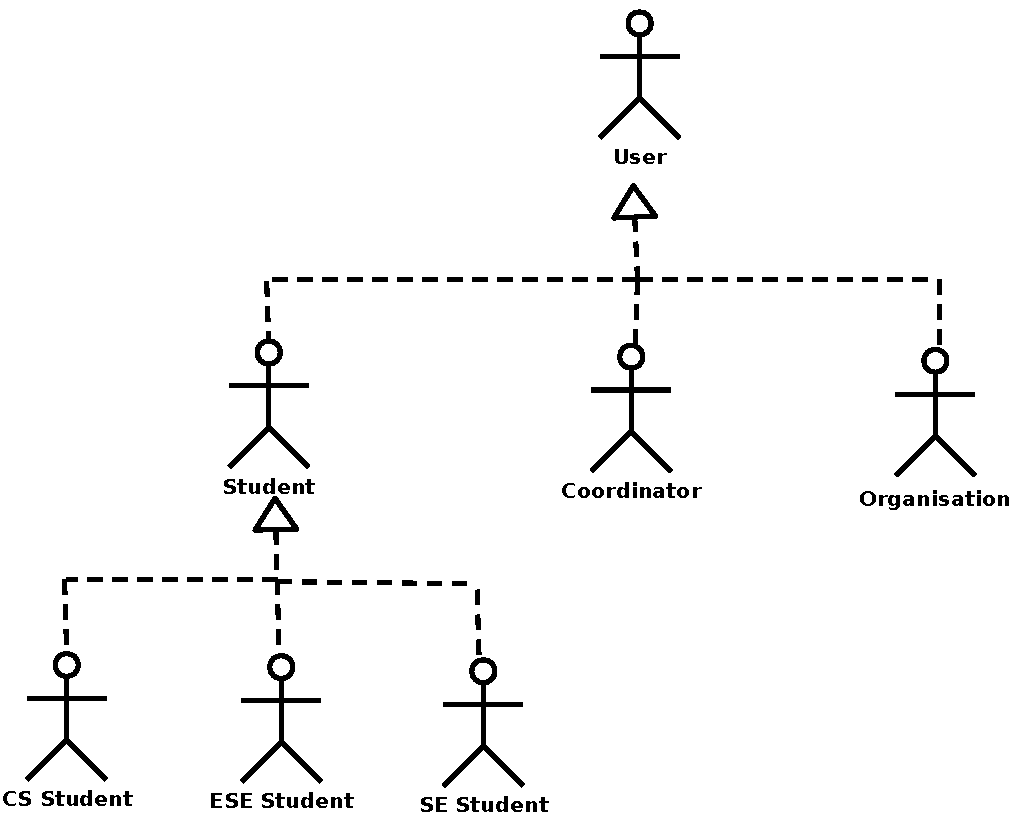
\includegraphics{"../Use Cases/Diagrams/Actors.png"}

The above diagram shows the actor roles present in the system:
\begin{itemize}
\item{\textbf{Student:}\ all students enrolled in the system who can apply for placements. This can be further broken down into SE and ESE students, who will have
different rules on what constitues a suitable placment.}
\item{\textbf{Coordinator: }\ the course coordinator will have privileges to approve and reject files, view student progress, etc.}
\item{\textbf{Organisation: }\ any group who advertises placements to the system. This may include external companies, intership schemes and university groups.}
\end{itemize}
%%%%%%%%%%%%%%%%%%%%%%%%%%%%%%%%%%%%%%%%%%%%%%%%%%%%%%%%%%%%%%%%%%%%%%%%%%%%%%

\subsection{Domain Model}
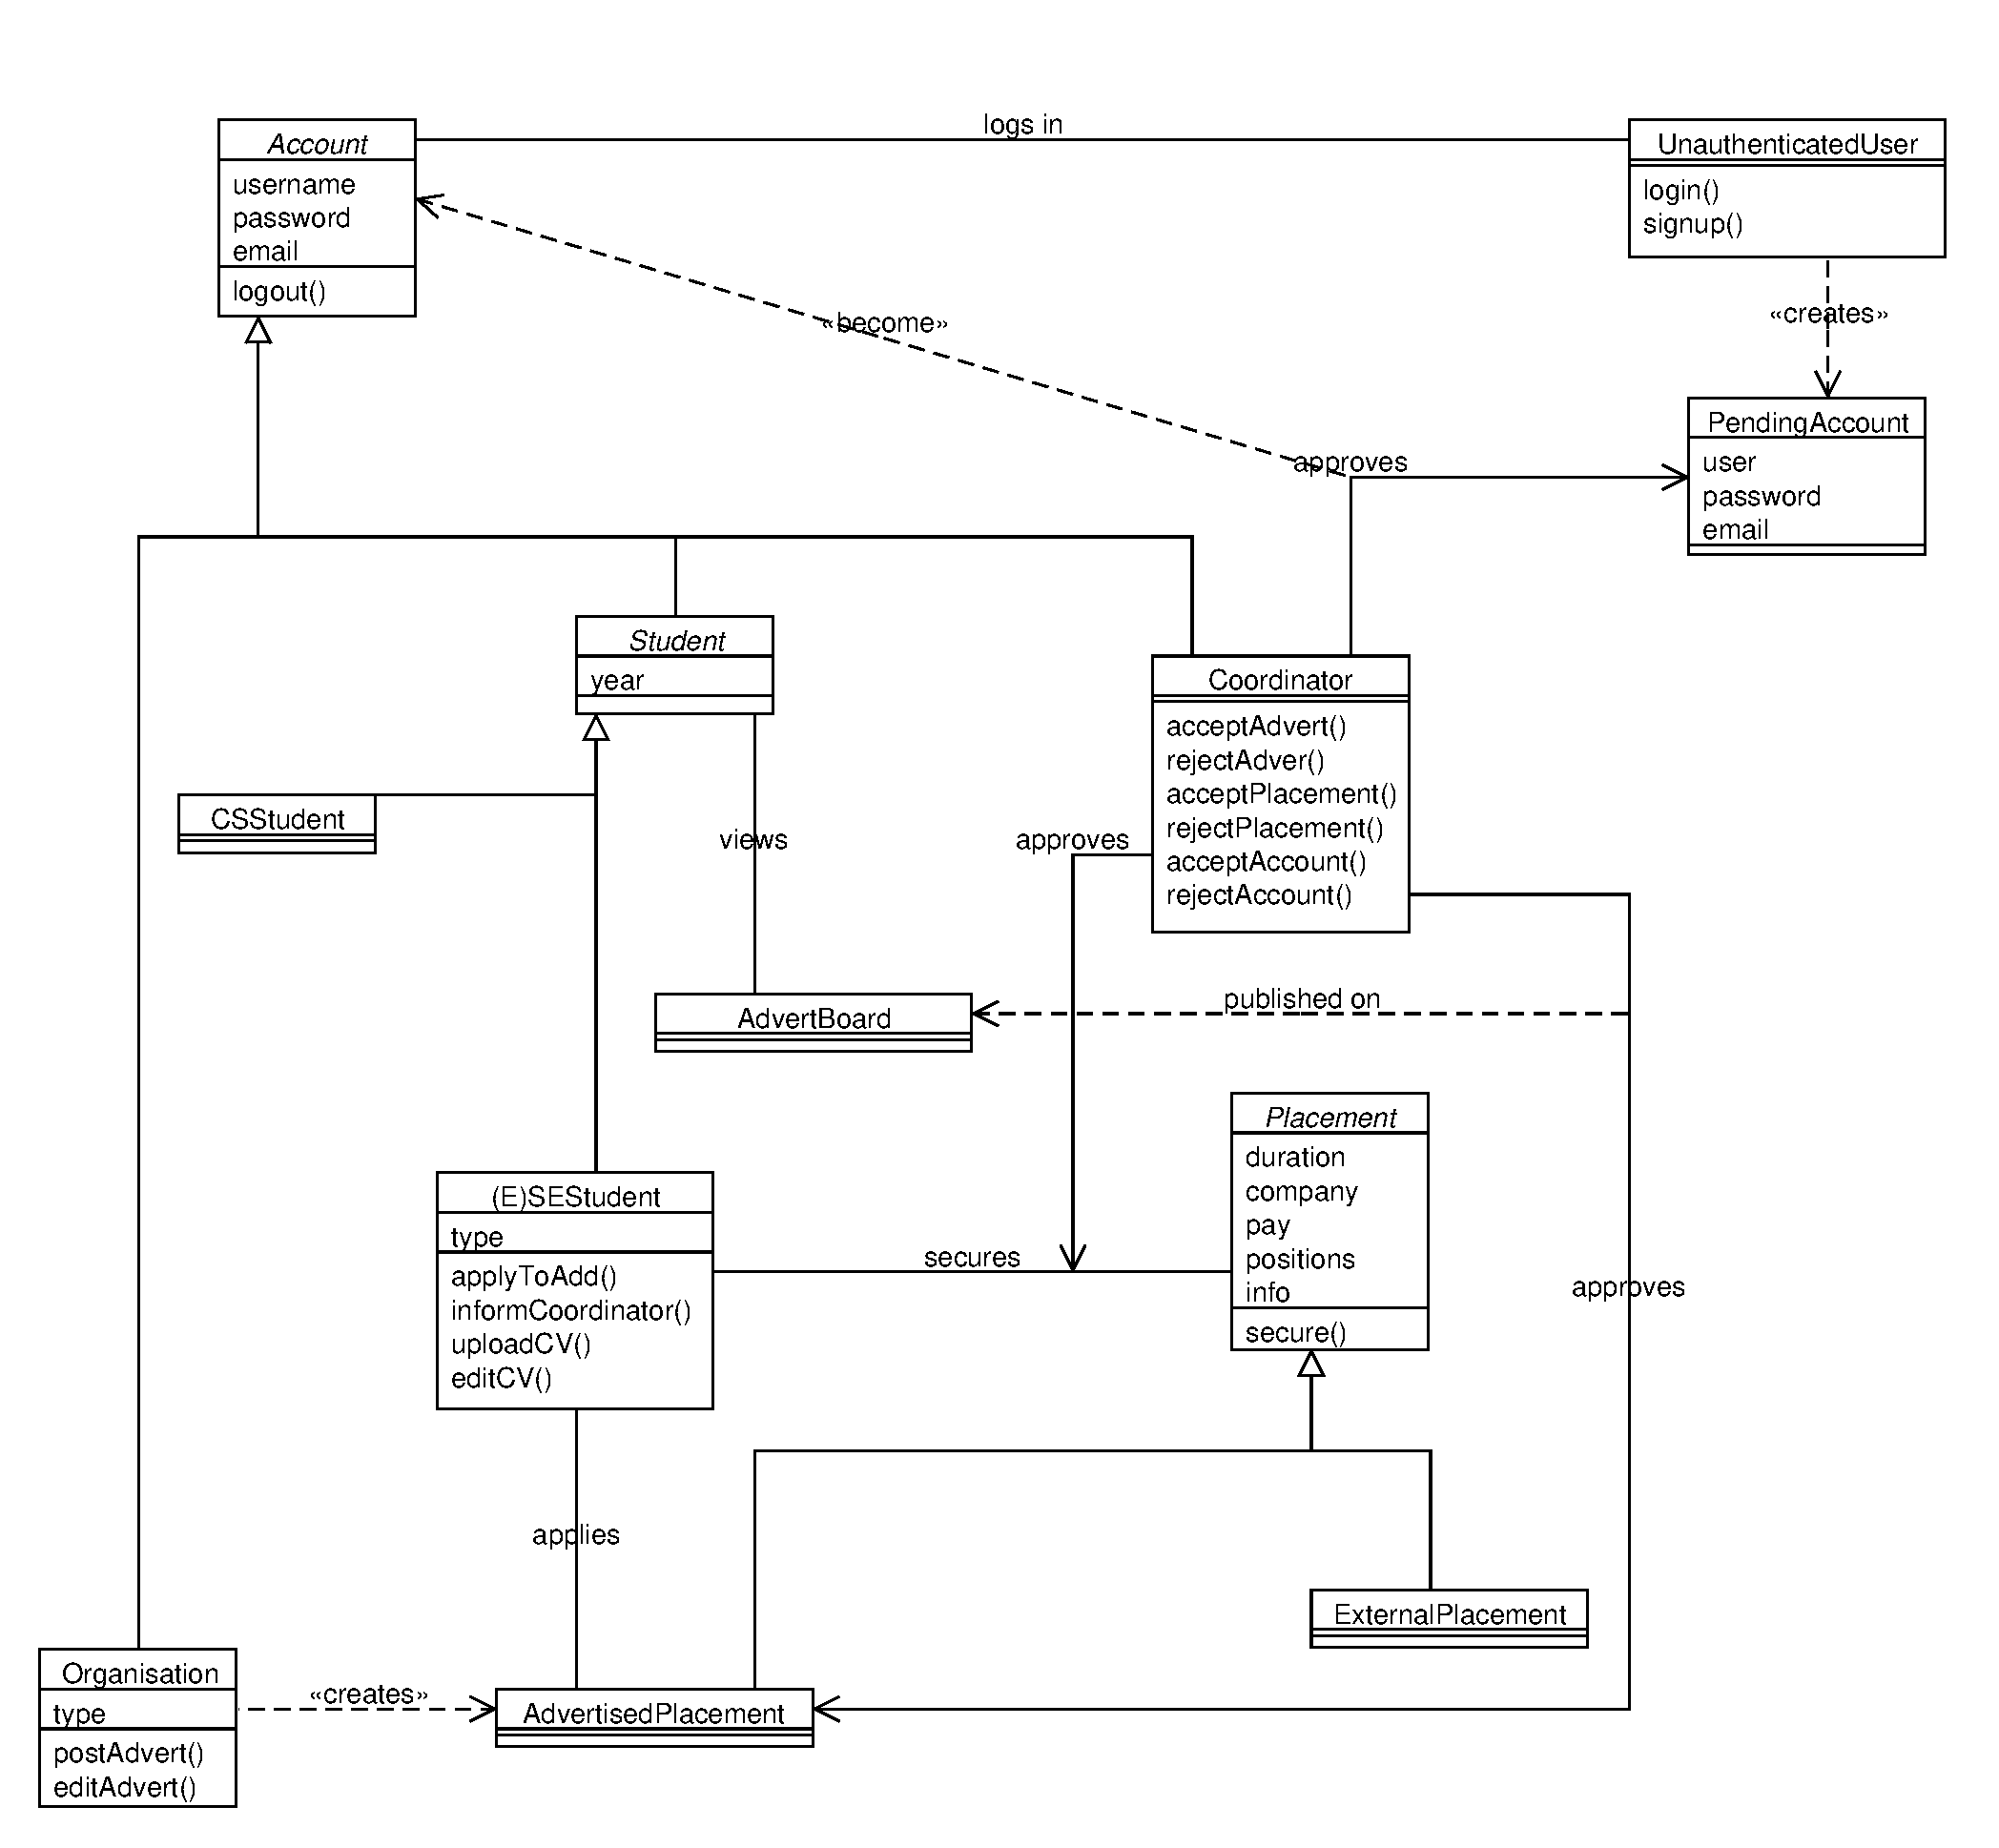
\includegraphics{"../Use Cases/domain_model_v1.pdf"}



%%%%%%%%%%%%%%%%%%%%%%%%%%%%%%%%%%%%%%%%%%%%%%%%%%%%%%%%%%%%%%%%%%%%%%%%%%%%%%

\section{Use Case Descriptions}
This section describes the key features which are required for the system. These can be broken into four categories as follows:\
\begin{itemize}
\item{\textbf{Utilities / Account Management\\
	\begin{itemize}
		\item{Login}
		\item{Account Creation}
		\item{Company Account Creation}
	\end{itemize}
\end{itemize}



%%%%%%%%%%%%%%%%%%%%%%%%%%%%%%%%%%%%%%%%%%%%%%%%%%%%%%%%%%%%%%%%%%%%%%%%%%%%%%

\section{Non Functional Requirements}

Describe the non-functional requirements for the system here, giving a
rationale (traceable to your requirements gathering) for each.  You
will need to think about how to group/structure requirements in this
section.

%%%%%%%%%%%%%%%%%%%%%%%%%%%%%%%%%%%%%%%%%%%%%%%%%%%%%%%%%%%%%%%%%%%%%%%%%%%%%%

\section{Summary}

Give a (very short) summary of the key aspects of the requirements
specification.

%%%%%%%%%%%%%%%%%%%%%%%%%%%%%%%%%%%%%%%%%%%%%%%%%%%%%%%%%%%%%%%%%%%%%%%%%%%%%%

\appendix

Some suggested appendices are included below.

Appendices should be used to include information not completely
necessary to the understanding of the main document.

\section{Glossary}

Definitions.

\section{Scenarios}

A collection of scenarios you developed to exercise and refine your
use cases.

\section{Stakeholder Interview Documentation}

Any evidence you gathered from stakeholders relevant to your
requirements description.  You don't need to include everything
verbatim here, but summary documents, for example, identifying the key
points you identified (particularly if they relate to requirements
conflicts) can be useful.

\section{Stakeholder Panel Documentation}

(see above)

%%%%%%%%%%%%%%%%%%%%%%%%%%%%%%%%%%%%%%%%%%%%%%%%%%%%%%%%%%%%%%%%%%%%%%%%%%%%%%

\end{document}

%%%%%%%%%%%%%%%%%%%%%%%%%%%%%%%%%%%%%%%%%%%%%%%%%%%%%%%%%%%%%%%%%%%%%%%%%%%%%%
